\documentclass[11pt,a4paper]{article}

% ---------------------------------------------------------------------------
% Packages
% ---------------------------------------------------------------------------
\usepackage[utf8]{inputenc}
\usepackage[T1]{fontenc}
\usepackage[english]{babel}
\usepackage[left=2cm, right=2cm, top=1.8cm, bottom=1.8cm]{geometry}
% REVISED (2026-10-28, margins 2): was \usepackage[left=2.5cm, right=2.5cm, top=2cm,
% bottom=2cm]{geometry} -- margins reduced again to gain space (25 -> 23 pages). The
% figures included with width=\textwidth now use width=0.94\textwidth, i.e. 16cm, the
% same physical size as before.
% REVISED (2026-10-28): was \usepackage[margin=2.5cm]{geometry} -- top and bottom
% margins reduced to 2cm to gain space for the text.
\usepackage{amsmath, amssymb, amsthm}
\usepackage{graphicx}
\usepackage{epstopdf}
\usepackage{float} % [H]: keep figures and tables exactly where they are in the text

% allow LaTeX a little extra stretch to avoid lines overflowing into the margin
\setlength{\emergencystretch}{2em}
\usepackage{booktabs}
\usepackage{array}
\usepackage{tikz}
\usetikzlibrary{arrows.meta}

% ---------------------------------------------------------------------------
% TikZ styles for small digraphs (edge i -> j: agent i is influenced by agent j)
% ---------------------------------------------------------------------------
\tikzset{
  agent/.style    = {circle, draw, inner sep=0pt, minimum size=4.5mm, font=\scriptsize},
  edge/.style     = {-{Stealth[length=1.6mm]}, thin},
  selfloop/.style = {-{Stealth[length=1.6mm]}, thin, loop above, looseness=6, min distance=4mm},
  weight/.style   = {font=\tiny, inner sep=1pt}
}
\usepackage{subcaption}
\usepackage[hidelinks]{hyperref}

% ---------------------------------------------------------------------------
% Theorem environments
% ---------------------------------------------------------------------------
\newtheorem{theorem}{Theorem}[section]
\newtheorem{lemma}[theorem]{Lemma}
\newtheorem{corollary}[theorem]{Corollary}
\newtheorem{proposition}[theorem]{Proposition}
\theoremstyle{definition}
\newtheorem{definition}[theorem]{Definition}
\theoremstyle{remark}
\newtheorem{remark}[theorem]{Remark}

% ---------------------------------------------------------------------------
% Title
% ---------------------------------------------------------------------------
\title{Title}
\author{Leonardo Luigi Pepe}
\date{\today}

\begin{document}

\maketitle

\begin{abstract}
Abstract.
\end{abstract}

\tableofcontents
\newpage

\section{Introduction}
\label{sec:intro}
% \input{intro/...}


\section{FDG}
\label{sec:fdg}

%2 pagine
\subsection{Introduction to the FDG model}
\label{subsec:fdg-intro}
% REVISED (2026-10-24): Theorems Consensus, Disagreement and Corollary Average consensus
% are now stated exactly as in the course slides (only the notation is adapted).

\subsubsection{The FDG model}
\label{subsubsec:fdg-model}

Consider a group of agents $V = \{1, 2, \dots, n\}$, where $x_i \in \mathbb{R}$ is the
opinion of agent $i$ on a given topic, and a weighted digraph
$G = (V, E, \{a_{ij}\}_{(i,j) \in E})$ describing who influences whom, with the
convention of Section~\ref{subsec:prelim}. In the
French--Harary--DeGroot (FDG) model~\cite{baggio_dt}, called French--DeGroot model
in~\cite{proskurnikov2017tutorial}, the new opinion of each agent is a weighted average
of the opinions of the agents it is influenced by,
% REVISED (2026-10-28, review): shortened; the edge convention is already stated in Section 1.1. Was:
% Consider a group of individuals $V = \{1, 2, \dots, n\}$, where $x_i \in \mathbb{R}$
% is the opinion that individual $i$ holds on a given topic. The influences among the
% individuals are described by a weighted digraph
% $G = (V, E, \{a_{ij}\}_{(i,j) \in E})$: following the convention of
% Section~\ref{subsec:prelim}, an edge $(i,j) \in E$, with weight $a_{ij} > 0$, means
% that individual $i$ is influenced by individual $j$.
%
% The French--Harary--DeGroot (FDG) model~\cite{baggio_dt}, called French--DeGroot
% model in~\cite{proskurnikov2017tutorial}, describes how each individual, or agent,
% updates its opinion: the new opinion is a weighted average of the opinions of the
% agents it is influenced by,
\begin{equation}\label{eq:fdg}
  x_i(k+1) = \sum_{j=1}^{n} a_{ij}\, x_j(k), \qquad \sum_{j=1}^{n} a_{ij} = 1,
\end{equation}
or, in vector form, $x(k+1) = A x(k)$, where $A$ is the weighted adjacency matrix
of $G$ (Definition~\ref{def:adjacency}). The constraint on the weights means that
$A$ is row-stochastic (Definition~\ref{def:row-stochastic}). In the terminology
of~\cite{baggio_dt}, the FDG model is a \emph{DT averaging system}.

Since $x(k) = A^k x(0)$, the asymptotic behaviour of the model is determined by the
powers of $A$. Three outcomes are possible:
\begin{itemize}
  \item \emph{no convergence}: $\lim_{k \to +\infty} x(k)$ does not exist for some
        $x(0)$; this happens when $A$ is not semi-convergent
        (Definition~\ref{def:semiconv}), e.g.\ when $A$ has an
        eigenvalue $\mu \neq 1$ with $|\mu| = 1$;
  \item \emph{consensus}: for every $x(0)$, $\lim_{k \to +\infty} x(k) = \alpha \mathbf{1}_n$
        for some $\alpha \in \mathbb{R}$, which depends on
        $x(0)$~\cite{proskurnikov2017tutorial};
% REVISED (2026-10-24): "for every x(0)" added to the consensus outcome, as in
% Definition 14 of the tutorial (consensus is a property of the model); the other two
% outcomes are unchanged (as in the course slides).
  \item \emph{disagreement}: $\lim_{k \to +\infty} x(k) = v$ with
        $v \neq \alpha \mathbf{1}_n$ for every $\alpha \in \mathbb{R}$.
\end{itemize}


\subsubsection{Consensus and social power}
\label{subsubsec:consensus}

The following theorem characterizes when the FDG model reaches a consensus. Its
condition (A3) involves the subgraph of globally reachable nodes, which is always
strongly connected~\cite{baggio_dt}, so that its periodicity is well defined
(Definition~\ref{def:periodic}).
% REVISED (2026-10-28, review): shortened (the justification of the strong connectivity is dropped). Was:
% The following theorem characterizes when the FDG model reaches a consensus. Its
% condition (A3) involves the subgraph of globally reachable nodes. This set of nodes is
% always strongly connected~\cite{baggio_dt}, since a walk between two globally reachable
% nodes only visits nodes that are themselves globally reachable. Hence its periodicity is well defined
% (Definition~\ref{def:periodic}).

\begin{theorem}[Consensus in DT averaging systems~\cite{baggio_dt}]
\label{thm:consensus}
Let $G$ be a weighted digraph with row-stochastic adjacency matrix $A$. The following
statements are equivalent:
\begin{itemize}
  \item[(A1)] the eigenvalue $1$ is simple and all other eigenvalues $\mu$ satisfy
              $|\mu| < 1$;
  \item[(A2)] $A$ is semi-convergent and
              $\lim_{k \to \infty} A^k = \mathbf{1}_n w^\top$ where
              $w \in \mathbb{R}^n$ satisfies $w \geq 0$,
              $\mathbf{1}_n^\top w = 1$, and $w^\top A = w^\top$;
  \item[(A3)] $G$ contains a globally reachable node and the subgraph of globally
              reachable nodes is aperiodic.
\end{itemize}
If any, and therefore all, of the previous conditions are satisfied, then
\begin{itemize}
  \item[(i)]  $w$ is the left dominant eigenvector of $A$ and $w_i > 0$ iff node $i$
              is globally reachable;
  \item[(ii)] the solution of the DT averaging system satisfies
              $\lim_{k \to \infty} x(k) = \big(w^\top x(0)\big)\mathbf{1}_n$.
\end{itemize}
\end{theorem}

\begin{corollary}[Average consensus~\cite{baggio_dt}]
\label{cor:average}
If $A$ is doubly-stochastic and (A3) holds, then
$w = \frac{1}{n}\mathbf{1}_n$ and
$\lim_{k \to +\infty} x(k) = \big(\frac{1}{n}\sum_{i=1}^{n} x_i(0)\big)\, \mathbf{1}_n$.
\end{corollary}

In Theorem~\ref{thm:consensus}, the left dominant eigenvector is the left eigenvector
associated with the dominant eigenvalue $\rho(A) = 1$
(Theorem~\ref{thm:stoch-spectrum})~\cite{baggio_matrix}.

\paragraph{Social power.}
The entry $w_i$ is called the \emph{social power} of agent $i$: it is the weight of
the initial opinion $x_i(0)$ in the final opinion of the group, i.e.\ in the consensus
value~\cite{proskurnikov2017tutorial}
\begin{equation}\label{eq:social-power}
  \lim_{k \to \infty} x_i(k) = w^\top x(0) = \sum_{j=1}^{n} w_j\, x_j(0)
  \qquad \text{for every agent } i.
\end{equation}
This definition requires a consensus: by (A2), all the rows of
$\lim_{k \to \infty} A^k = \mathbf{1}_n w^\top$ are equal to $w^\top$, so a single vector
describes the whole group. Without a consensus, as in Theorem~\ref{thm:disagreement},
the rows of the limit matrix differ, each agent ends at its own weighted average of the
initial opinions, and no single vector plays the role of $w$.
% REVISED (2026-10-28, review): shortened, same content. Was:
% This definition requires a consensus. By (A2), $\lim_{k \to \infty} A^k = \mathbf{1}_n w^\top$: all the rows of the
% limit matrix are equal to $w^\top$, so every agent ends at the same weighted average
% $w^\top x(0)$ of the initial opinions, and a single vector $w$ describes the whole
% group. Without a consensus, as in Theorem~\ref{thm:disagreement}, the limit matrix
% still exists, but its rows are not all equal, otherwise every agent would end at the
% same value for every $x(0)$: each agent ends at its own weighted average of the
% initial opinions, so the weight of $x_j(0)$ depends on the agent, and no single vector
% plays the role of $w$.
% REVISED (2026-10-24): added why the social power requires a consensus (rows of the
% limit matrix all equal to w^T under (A2), not all equal in the disagreement case).

Point (i) has a direct social interpretation: the consensus value is the same for
every agent, so the initial opinion of agent $i$ can enter it only if it reaches
\emph{all} the agents, i.e.\ if $i$ is globally reachable. Hence the consensus value
depends only on the initial opinions of the globally reachable agents.
% REVISED (2026-10-28, review): shortened, same content. Was:
% Point (i) has a direct social interpretation. Since the consensus value
% $w^\top x(0)$ is the same for every agent, the initial opinion of agent $i$ can
% contribute to it only if it reaches \emph{all} the agents. If $i$ is not globally
% reachable, there is at least one agent that is influenced by $i$ neither directly
% nor through intermediaries: the opinion of $i$ never reaches that agent, so it
% cannot enter the common value, and $w_i = 0$. Conversely, the opinion of a globally
% reachable agent reaches the whole group and has a positive weight. Hence the
% consensus value depends only on the initial opinions of the globally reachable
% agents.

Among the globally reachable agents, the social power depends on their position in the
network, and it can be regarded as a centrality measure~\cite{proskurnikov2017tutorial}.
For instance, in the model of French with $n = 3$ agents and
\[
  A = \begin{bmatrix} 1/2 & 1/2 & 0 \\ 1/3 & 1/3 & 1/3 \\ 0 & 1/2 & 1/2 \end{bmatrix},
\]
all agents are globally reachable, but agent~$2$, the only one listened to by all the
others, has the largest social power, $w = (2/7,\, 3/7,\, 2/7)^\top$~\cite{proskurnikov2017tutorial}.
% REVISED (2026-10-28, review): shortened (the description of who listens to whom can be read on the matrix). Was:
% agents~$1$ and~$3$ listen to themselves and to agent~$2$, while agent~$2$ listens to
% everybody. All agents are globally reachable, but agent~$2$, the only one listened to by
% all the others, has the largest social power:
% $w = (2/7,\, 3/7,\, 2/7)^\top$~\cite{proskurnikov2017tutorial}.


\subsubsection{Disagreement}
\label{subsubsec:disagreement}

Theorem~\ref{thm:consensus} requires a single globally reachable group, i.e.\ a
unique sink in the condensation digraph $C(G)$. We now consider the case in which
$C(G)$ has $n_s \geq 2$ sinks. Each sink is a strongly connected component, so its
periodicity is well defined (Definition~\ref{def:periodic}).

\begin{theorem}[Disagreement in DT averaging systems~\cite{baggio_dt}]
\label{thm:disagreement}
Let $G$ be a weighted digraph with row-stochastic adjacency matrix $A$. Assume that
the condensation digraph $C(G)$ has $n_s \geq 2$ sinks. The following statements are
equivalent:
\begin{itemize}
  \item[(A1)] the eigenvalue $1$ is semi-simple with multiplicity $n_s$ and all other
              eigenvalues $\mu$ satisfy $|\mu| < 1$;
  \item[(A2)] $A$ is semi-convergent;
  \item[(A3)] each sink of $C(G)$ is aperiodic.
\end{itemize}
If any, and therefore all, of the previous conditions are satisfied, then the solution
of the DT averaging system satisfies
\[
  \lim_{k \to \infty} x(k) = v \neq \alpha \mathbf{1}_n, \quad \alpha \in \mathbb{R}.
\]
\end{theorem}

The final opinions can be described group by group. The agents of a sink are not
influenced by anyone outside it, so each sink evolves as an FDG model on its own and,
being aperiodic, reaches an internal consensus that depends only on the initial
opinions of its members; every agent outside the sinks converges to a convex
combination of the consensus values of the sinks~\cite{baggio_dt}. In social terms, a
sink is a closed group that listens only to itself, and the agents in between settle
on an intermediate opinion: the disagreement is bounded by the smallest and the largest
consensus value of the sinks.
% REVISED (2026-10-28, review): two paragraphs merged, same content. Was:
% The final opinions can be described group by group. The agents of a sink are not
% influenced by anyone outside the sink, so each sink evolves as an FDG model on its own
% and, being aperiodic, reaches an internal consensus that depends only on the initial
% opinions of its members. Every agent outside the sinks converges instead to a convex
% combination of the consensus values of the sinks~\cite{baggio_dt}.
%
% In social terms, a sink is a closed group that listens only to itself, and two closed
% groups never influence each other: each of them keeps its own consensus value. The
% agents in between listen, directly or through intermediaries, to several closed
% groups and settle on an intermediate opinion between their consensus values. As a
% consequence, the disagreement is bounded: every final opinion lies between
% the smallest and the largest consensus value of the sinks.


\subsubsection{Rosetta stone}
\label{subsubsec:rosetta}

Table~\ref{tab:rosetta}, the so-called \emph{Rosetta stone}~\cite{baggio_dt},
summarizes all the possible behaviours of the FDG model: it translates each property
of the row-stochastic matrix $A$ into a property of the digraph $G$ and into the
asymptotic outcome, with an example for each case; the translation between $A$ and $G$
comes from Theorems~\ref{thm:irreducible} and~\ref{thm:primitive} in cases (i)--(ii),
and from Theorems~\ref{thm:consensus} and~\ref{thm:disagreement} in cases
(iii)--(iv). In case~(i) both agents are
globally reachable and $A$ is doubly-stochastic, so by Corollary~\ref{cor:average} the
group agrees on the average of the initial opinions. In case~(iii) agent~$1$ is
stubborn (Definition~\ref{def:stubborn}) and is the only globally reachable agent:
$w = (1, 0)^\top$ and the group agrees on $x_1(0)$. In case~(iv) both agents are
stubborn: each of them is an aperiodic sink of $C(G)$, and every agent keeps its
initial opinion (Theorem~\ref{thm:disagreement}).
% REVISED (2026-10-28, review): shortened; cases (iii) and (iv) are now read as one and two stubborn agents, the thread of Section 2.2; Theorems 1.12 and 1.13, never cited before, are now cited for cases (i)-(ii). Was:
% The results of this section, together with the consensus and disagreement theorems
% above, classify all the possible behaviours of the FDG model. The classification is
% summarized in Table~\ref{tab:rosetta}, the so-called \emph{Rosetta stone}~\cite{baggio_dt}, which
% translates each property of the row-stochastic matrix $A$ into a property of the
% digraph $G$ and into the corresponding asymptotic outcome; for each case, the table
% also reports an example digraph, its matrix and its spectrum.
%
% The two consensus cases illustrate Theorem~\ref{thm:consensus}. In case~(i) both
% agents are globally reachable and $A$ is doubly-stochastic, so by
% Corollary~\ref{cor:average} $w = (1/2, 1/2)^\top$ and the group agrees on the average
% $\big(x_1(0) + x_2(0)\big)/2$. In case~(iii) agent~$2$ is influenced by agent~$1$
% but not vice versa, so only agent~$1$ is globally reachable: $w = (1, 0)^\top$ and
% the group agrees on $x_1(0)$, whatever the initial opinion of agent~$2$.
%
% Case~(iv) illustrates Theorem~\ref{thm:disagreement} in its simplest form: each agent
% is influenced only by itself, so each agent is a sink of $C(G)$ ($n_s = 2$), both sinks
% are aperiodic thanks to the self-loops, and every agent keeps its initial opinion,
% $x(k) = x(0)$ for all $k$.

\begin{table}[H]
  \centering
  \small
  \renewcommand{\arraystretch}{1.6}
  \begin{tabular}{@{}c c c c >{\raggedright\arraybackslash}m{4.4cm} l@{}}
    \toprule
    Case & Example digraph & $A$ & $\operatorname{spec}(A)$ & Property of $A$ / of $G$ & Outcome \\
    \midrule
    (i)
      & 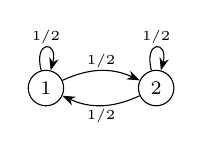
\begin{tikzpicture}[baseline=-0.6ex]
          \node[agent] (a) at (0,0) {1}; \node[agent] (b) at (1.4,0) {2};
          \draw[edge] (a) to[bend left=25] node[weight, above] {1/2} (b);
          \draw[edge] (b) to[bend left=25] node[weight, below] {1/2} (a);
          \draw[selfloop] (a) to node[weight, above] {1/2} (a);
          \draw[selfloop] (b) to node[weight, above] {1/2} (b);
        \end{tikzpicture}
      & $\left[\begin{smallmatrix} 1/2 & 1/2 \\ 1/2 & 1/2 \end{smallmatrix}\right]$
      & $\{1,\, 0\}$
      & $A$ primitive / $G$ strongly connected and aperiodic
      & consensus \\
    (ii)
      & 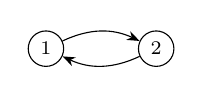
\begin{tikzpicture}[baseline=-0.6ex]
          \node[agent] (a) at (0,0) {1}; \node[agent] (b) at (1.4,0) {2};
          \draw[edge] (a) to[bend left=25] (b);
          \draw[edge] (b) to[bend left=25] (a);
        \end{tikzpicture}
      & $\left[\begin{smallmatrix} 0 & 1 \\ 1 & 0 \end{smallmatrix}\right]$
      & $\{1,\, -1\}$
      & $A$ irreducible, not primitive / $G$ strongly connected and periodic
      & no convergence \\
    (iii)
      & 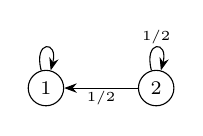
\begin{tikzpicture}[baseline=-0.6ex]
          \node[agent] (a) at (0,0) {1}; \node[agent] (b) at (1.4,0) {2};
          \draw[edge] (b) to node[weight, below] {1/2} (a);
          \draw[selfloop] (a) to (a);
          \draw[selfloop] (b) to node[weight, above] {1/2} (b);
        \end{tikzpicture}
      & $\left[\begin{smallmatrix} 1 & 0 \\ 1/2 & 1/2 \end{smallmatrix}\right]$
      & $\{1,\, 1/2\}$
      & $1$ simple and strictly dominant, $A$ not primitive / $C(G)$ has a unique sink, which is aperiodic
      & consensus \\
    (iv)
      & 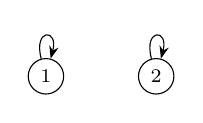
\begin{tikzpicture}[baseline=-0.6ex]
          \node[agent] (a) at (0,0) {1}; \node[agent] (b) at (1.4,0) {2};
          \draw[selfloop] (a) to (a);
          \draw[selfloop] (b) to (b);
        \end{tikzpicture}
      & $\left[\begin{smallmatrix} 1 & 0 \\ 0 & 1 \end{smallmatrix}\right]$
      & $\{1,\, 1\}$
      & $1$ semi-simple but not simple, strictly dominant / $C(G)$ has at least two sinks, all aperiodic
      & disagreement \\
    (v)
      & 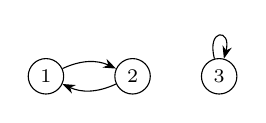
\begin{tikzpicture}[baseline=-0.6ex]
          \node[agent] (a) at (0,0) {1}; \node[agent] (b) at (1.1,0) {2};
          \node[agent] (c) at (2.2,0) {3};
          \draw[edge] (a) to[bend left=25] (b);
          \draw[edge] (b) to[bend left=25] (a);
          \draw[selfloop] (c) to (c);
        \end{tikzpicture}
      & $\left[\begin{smallmatrix} 0 & 1 & 0 \\ 1 & 0 & 0 \\ 0 & 0 & 1 \end{smallmatrix}\right]$
      & $\{1,\, 1,\, -1\}$
      & $1$ not strictly dominant / $G$ not strongly connected, at least one sink of $C(G)$ is periodic
      & no convergence \\
    \bottomrule
  \end{tabular}
  \caption{Rosetta stone of the FDG model $x(k+1) = A x(k)$, with $A$ row-stochastic:
  for each case, an example digraph (unlabelled edges have weight $1$), its matrix
  $A$, the spectrum of $A$, the general property of $A$ and of $G$, and the outcome. Cases (i)--(iv)
  and the examples follow~\cite{baggio_dt}; the properties of case (v),
  left blank in the slides, follow from~\cite{proskurnikov2017tutorial}.}
  \label{tab:rosetta}
\end{table}


%4 pagine
\subsection{Stubbornness and social power in the FDG model}
\label{subsec:fdg-stub}

In the FDG model the simplest way to account for stubbornness is the self-weight
$a_{ii}$, i.e.\ the weight of the self-loop of agent $i$. This section studies how
self-weights, and stubborn agents in particular, affect the two aspects introduced in
Section~\ref{subsec:fdg-intro}: whether the group reaches an agreement, and how the
social power is distributed among the agents.

All the examples use the two networks of Figure~\ref{fig:networks}, both with $n = 6$
agents: in the \emph{directed cycle} each agent is influenced only by the next one,
$a_{i,i+1} = 1$; in the \emph{bidirectional ring} by its two neighbours,
$a_{i,i-1} = a_{i,i+1} = 1/2$ (indices modulo $6$). Socially, in the first network
everyone listens to a single person, in the second to the two people next to them.
Without self-loops both digraphs are strongly connected and periodic, with period $6$
for the directed cycle and $2$ for the bidirectional ring, whose cycles all have even
length: neither network reaches an agreement (case~(ii) of Table~\ref{tab:rosetta}).
Both matrices are doubly-stochastic, so $w = \frac{1}{6}\mathbf{1}_6$ is the left
eigenvector associated with the eigenvalue $1$: no agent is favoured by the structure
of the network, and any asymmetry in the social power will be due only to the
self-weight added to agent~$1$.
% REVISED (2026-10-28, review): shortened, same content. Was:
% All the examples use the two networks of Figure~\ref{fig:networks}, both with $n = 6$
% agents. In the \emph{directed cycle} each agent is influenced only by the next one,
% $a_{i,i+1} = 1$; in the \emph{bidirectional ring} each agent is influenced by its two
% neighbours with equal weights, $a_{i,i-1} = a_{i,i+1} = 1/2$ (indices modulo $6$).
% Socially, in the first network everyone listens to a single person, while in the second
% everyone listens to the two people next to them. Without self-loops both digraphs are
% strongly connected and periodic: the directed cycle has a single cycle, of length $6$,
% while every cycle of the bidirectional ring has even length, so its period is $2$.
% Hence neither network reaches an agreement (case~(ii) of Table~\ref{tab:rosetta}).
% Moreover, both matrices are doubly-stochastic, so $w = \frac{1}{6}\mathbf{1}_6$ is the
% left eigenvector associated with the eigenvalue $1$: no agent is favoured by the
% structure of the network, and any asymmetry in the social power will be due only to
% the self-weight added to agent~$1$.

\begin{figure}[H]
  \centering
  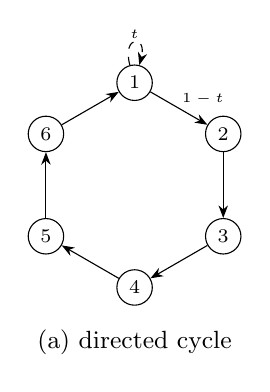
\begin{tikzpicture}[baseline=(c.base)]
    \foreach \i in {1,...,6} {
      \node[agent] (d\i) at ({90-60*(\i-1)}:1.3) {\i};
    }
    \node (c) at (0,0) {};
    \foreach \i/\j in {2/3,3/4,4/5,5/6,6/1} {
      \draw[edge] (d\i) -- (d\j);
    }
    \draw[edge] (d1) -- node[weight, above right] {$1-t$} (d2);
    \draw[selfloop, dashed] (d1) to node[weight, above] {$t$} (d1);
    % REVISED (2026-10-28): the edge 1 -> 2 is now drawn separately with its weight 1-t
    % (was part of the \foreach list 1/2,2/3,...,6/1).
    \node at (0,-2.0) {\small (a) directed cycle};
  \end{tikzpicture}
  \hspace{1.5cm}
  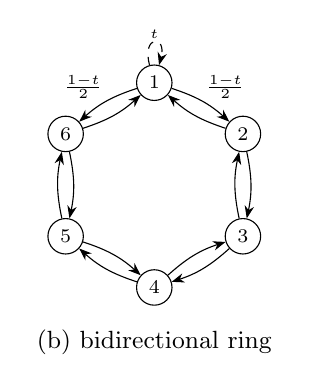
\begin{tikzpicture}[baseline=(c.base)]
    \foreach \i in {1,...,6} {
      \node[agent] (b\i) at ({90-60*(\i-1)}:1.3) {\i};
    }
    \node (c) at (0,0) {};
    \foreach \i/\j in {2/3,3/4,4/5,5/6} {
      \draw[edge] (b\i) to[bend left=12] (b\j);
      \draw[edge] (b\j) to[bend left=12] (b\i);
    }
    \draw[edge] (b2) to[bend left=12] (b1);
    \draw[edge] (b6) to[bend right=12] (b1);
    \draw[edge] (b1) to[bend left=12] node[weight, above right] {$\frac{1-t}{2}$} (b2);
    \draw[edge] (b1) to[bend right=12] node[weight, above left] {$\frac{1-t}{2}$} (b6);
    \draw[selfloop, dashed] (b1) to node[weight, above] {$t$} (b1);
    % REVISED (2026-10-28): the edges 1 -> 2 and 1 -> 6 are now drawn separately with
    % their weight (1-t)/2 (were part of the \foreach list 1/2,...,6/1).
    \node at (0,-2.0) {\small (b) bidirectional ring};
  \end{tikzpicture}
  \caption{The two networks used in Sections~\ref{subsec:fdg-stub}
  and~\ref{sec:fj}. An edge $i \to j$ means that agent $i$ is influenced by agent $j$.
  In (a) all edges have weight $1$, in (b) all edges have weight $1/2$. The dashed
  self-loop of agent~$1$, of weight $t$, is the only modification considered: the
  other edges of agent~$1$ are scaled by $1-t$, as marked
  (equation~\eqref{eq:self-weight}).}
  % REVISED (2026-10-28): added "as marked" (the weights of the edges of agent 1 are now
  % written on the figure).
  \label{fig:networks}
\end{figure}

\subsubsection{Modelling stubbornness: self-weights and stubborn agents}
\label{subsubsec:fdg-stub-model}

The self-weight $a_{ii}$ is the weight that agent $i$ gives to its own \emph{current}
opinion~\cite{bullo2024lns}; it indicates how open the agent is to the opinions of the
others~\cite{proskurnikov2017tutorial}. An agent with $a_{ii} = 0$ is open-minded and
relies completely on the others; an agent with a positive self-weight changes its
opinion more slowly, but it still moves towards the opinions it listens to. In social
terms, a self-weight is a form of inertia, not an anchor to a fixed opinion.

\begin{definition}[Stubbornness~\cite{proskurnikov2017tutorial}]
\label{def:stubborn}
% REVISED (2026-10-24): definition now exactly as Definition 16 of the tutorial; the
% FDG characterization (a_ii = 1) is moved to the text below.
An agent is said to be \emph{stubborn} if its opinion remains unchanged independent
of the others' opinions.
\end{definition}

If the opinions obey the FDG model, then agent $i$ is stubborn, $x_i(k) \equiv x_i(0)$,
if and only if $a_{ii} = 1$~\cite{proskurnikov2017tutorial} (and hence $a_{ij} = 0$
for all $j \neq i$, since $A$ is row-stochastic).

Stubbornness is therefore the extreme case of the self-weight, and there is no
intermediate degree of it: an agent with $0 < a_{ii} < 1$ is not stubborn, it only has
a positive self-weight.

In the digraph, a stubborn agent has no edges towards the other agents: it is
influenced by nobody, while the agents that listen to it keep doing so. Hence it forms
a strongly connected component made of a single node, which is a sink of $C(G)$ and is
aperiodic because of its self-loop. If, in addition, every agent is influenced by the
stubborn agent $i$, directly or through intermediaries, then $i$ is the only globally
reachable node, and Theorem~\ref{thm:consensus} gives $w = e_i$: the whole group
converges to the initial opinion of the stubborn agent (see
also~\cite{proskurnikov2017tutorial}).

To move continuously from no self-weight to stubbornness, we modify only the row of
agent~$1$. Given a row-stochastic matrix $A$ with $a_{11} = 0$, as in both networks of
Figure~\ref{fig:networks}, we replace its first row by
\begin{equation}\label{eq:self-weight}
  a_1(t)^\top = (1-t)\, a_1^\top + t\, e_1^\top, \qquad t \in [0,1],
\end{equation}
where $e_1$ is the first vector of the canonical basis, leaving the other rows
unchanged: agent~$1$ gives weight $t$ to itself and splits the remaining weight $1-t$
among the agents it listened to before, in the same proportions, as marked in
Figure~\ref{fig:networks}. Thus $t = a_{11}$: $t = 0$ is the original network and
$t = 1$ makes agent~$1$ stubborn. In the following we consider $t = 0$, $1/2$ and $1$.
% REVISED (2026-10-28, review): shortened; the explicit first rows are now written on Figure 1. Was:
% where $e_1$ is the first vector of the canonical basis, and leave the other rows
% unchanged. Agent~$1$ gives weight $t$ to itself and splits the
% remaining weight $1-t$ among the agents it listened to before, in the same
% proportions. The parameter $t$ is thus the self-weight $a_{11}$: $t = 0$ is the
% original network, $0 < t < 1$ gives agent~$1$ a positive self-weight, and $t = 1$
% makes agent~$1$ stubborn. For the directed cycle the first row becomes
% $(t,\, 1-t,\, 0,\, 0,\, 0,\, 0)$; for the bidirectional ring it becomes
% $(t,\, \frac{1-t}{2},\, 0,\, 0,\, 0,\, \frac{1-t}{2})$. In the following we consider
% the three values $t = 0$, $t = 1/2$ and $t = 1$.

\subsubsection{Self-weights, stubbornness and convergence}
\label{subsubsec:fdg-stub-conv}

The three values of $t$ correspond to three different cases of the Rosetta stone.
\begin{itemize}
  \item $t = 0$: both digraphs are strongly connected and periodic, so neither
        network converges (case~(ii)).
  \item $0 < t < 1$: agent~$1$ still listens to its neighbours with total weight
        $1-t > 0$, so the digraph stays strongly connected, and the self-loop of
        agent~$1$ is a cycle of length $1$, so the digraph becomes aperiodic. By
        Corollary~\ref{cor:primitive-selfloop} the matrix is primitive, and the group reaches a
        consensus (case~(i)).
  \item $t = 1$: agent~$1$ is stubborn and influences every other agent through the
        cycle, so it is the only globally reachable node
        (Section~\ref{subsubsec:fdg-stub-model}) and the group reaches a consensus on
        $x_1(0)$ (case~(iii)).
% REVISED (2026-10-28, review): shortened, same content. Was:
%   \item $t = 1$: agent~$1$ is stubborn. In both networks every other agent is
%         influenced by agent~$1$ through the cycle, directly or through intermediaries,
%         so by the discussion in Section~\ref{subsubsec:fdg-stub-model} agent~$1$ is the
%         only sink of $C(G)$ and the only globally reachable node, so the group reaches a consensus on its initial
%         opinion $x_1(0)$ (case~(iii)).
\end{itemize}

The same picture can be read on the spectrum of $A(t)$. For $t = 0$ the spectrum is the
set of the sixth roots of unity for the directed cycle and
$\{1, \frac{1}{2}, \frac{1}{2}, -\frac{1}{2}, -\frac{1}{2}, -1\}$ for the bidirectional
ring: in both cases some eigenvalues different from $1$ lie on the unit circle, and
they cause the oscillations. For $t > 0$ all the eigenvalues different from $1$ lie
strictly inside the unit disk, and the group converges; for $t = 1/2$ the largest of
their moduli is $\approx 0.92$ on the directed cycle and $\approx 0.90$ on the
bidirectional ring. For $t = 1$ the directed cycle is left with the eigenvalue $0$, of
multiplicity $5$, which is why its consensus is reached in a finite number of steps.
% REVISED (2026-10-28, review): the characteristic polynomials and the lists of eigenvalues are summarized (FDG part to be kept essential); the moduli 0.92 and 0.90 are those of the removed lists for t = 1/2. Was:
% The same picture can be read on the spectrum of the matrix. For the directed cycle the
% characteristic polynomial is
% \[
%   p(\lambda) = (\lambda - 1)\,\big[\lambda^5 + (1-t)(\lambda^4 + \lambda^3 + \lambda^2
%   + \lambda + 1)\big].
% \]
% Apart from $\lambda_1 = 1$, the eigenvalues are the roots of a polynomial of degree $5$,
% which for a generic $t$ have no closed-form expression; for the three values of $t$
% they are
% \begin{itemize}
%   \item $t = 0$: $\lambda_1 = 1$, $\lambda_{2,3} = \frac{1}{2} \pm \frac{\sqrt{3}}{2}\,i$,
%         $\lambda_{4,5} = -\frac{1}{2} \pm \frac{\sqrt{3}}{2}\,i$, $\lambda_6 = -1$
%         (the sixth roots of unity, all on the unit circle);
%   \item $t = 1/2$: $\lambda_1 = 1$, $\lambda_{2,3} \approx 0.535 \pm 0.751\,i$,
%         $\lambda_{4,5} \approx -0.373 \pm 0.759\,i$, $\lambda_6 \approx -0.823$;
%   \item $t = 1$: $\lambda_1 = 1$, $\lambda_2 = \dots = \lambda_6 = 0$.
% \end{itemize}
% For the bidirectional ring the characteristic polynomial is
% \[
%   p(\lambda) = (\lambda - 1)\big(\lambda - \tfrac{1}{2}\big)
%   \big(\lambda + \tfrac{1}{2}\big)\Big[\lambda^3 + (1-t)\lambda^2
%   - \tfrac{2t+1}{4}\,\lambda + \tfrac{t-1}{4}\Big].
% \]
% The eigenvalues $1$ and $\pm\frac{1}{2}$ do not depend on $t$, while the other three are
% the roots of the cubic factor, whose closed-form expression in $t$ is too involved to be
% informative; for the three values of $t$ the eigenvalues are
% \begin{itemize}
%   \item $t = 0$: $\lambda_1 = 1$, $\lambda_{2,3} = \frac{1}{2}$,
%         $\lambda_{4,5} = -\frac{1}{2}$, $\lambda_6 = -1$ (on the unit circle);
%   \item $t = 1/2$: $\lambda_1 = 1$, $\lambda_2 \approx 0.623$, $\lambda_3 = \frac{1}{2}$,
%         $\lambda_4 \approx -0.223$, $\lambda_5 = -\frac{1}{2}$, $\lambda_6 \approx -0.901$;
%   \item $t = 1$: $\lambda_1 = 1$, $\lambda_2 = \frac{\sqrt{3}}{2}$,
%         $\lambda_3 = \frac{1}{2}$, $\lambda_4 = 0$, $\lambda_5 = -\frac{1}{2}$,
%         $\lambda_6 = -\frac{\sqrt{3}}{2}$.
% \end{itemize}
% In both networks, for $t = 0$ some eigenvalues different from $1$ lie on the unit
% circle, and they cause the oscillations; for $t > 0$ all the eigenvalues different
% from $1$ lie strictly inside the unit disk, and the group converges. For $t = 1$ the
% directed cycle is left with the eigenvalue $0$ only, which is why its convergence is
% reached in a finite number of steps.

Figure~\ref{fig:fdg-conv} shows the opinions $x_i(k)$ in the six cases. For $t = 0$
the opinions keep rotating along the directed cycle and oscillating between two
configurations on the bidirectional ring. For $t = 1/2$ both networks reach a consensus
on a weighted average of all the initial opinions (Section~\ref{subsubsec:fdg-stub-power}).
For $t = 1$ both reach $x_1(0)$, in different ways: in the directed cycle the opinion of
agent~$1$ is copied backwards along the chain, one agent per step, and the consensus is
reached after $n - 1 = 5$ steps; in the bidirectional ring the opinions approach
$x_1(0)$ gradually, the neighbours of agent~$1$ first.
% REVISED (2026-10-28, review): shortened, same content. Was:
% Figure~\ref{fig:fdg-conv} shows the opinions $x_i(k)$ in the six cases. For $t = 0$
% the opinions keep rotating along the directed cycle and keep oscillating between two
% configurations on the bidirectional ring. For $t = 1/2$ both networks reach a consensus
% whose value is a weighted average of all the initial opinions, with weights given by
% the social power (Section~\ref{subsubsec:fdg-stub-power}). For $t = 1$ both networks
% reach a consensus on $x_1(0)$, but in different ways. In the directed cycle every agent
% other than agent~$1$ simply copies the opinion of the next agent, so the opinion of
% agent~$1$ travels backwards along the chain, one agent per step, and the consensus is
% reached exactly after $n - 1 = 5$ steps. In the bidirectional ring every agent averages
% the opinions of its two neighbours, so the opinions approach $x_1(0)$ gradually, the
% neighbours of agent~$1$ first.

\begin{figure}[H]
  \centering
  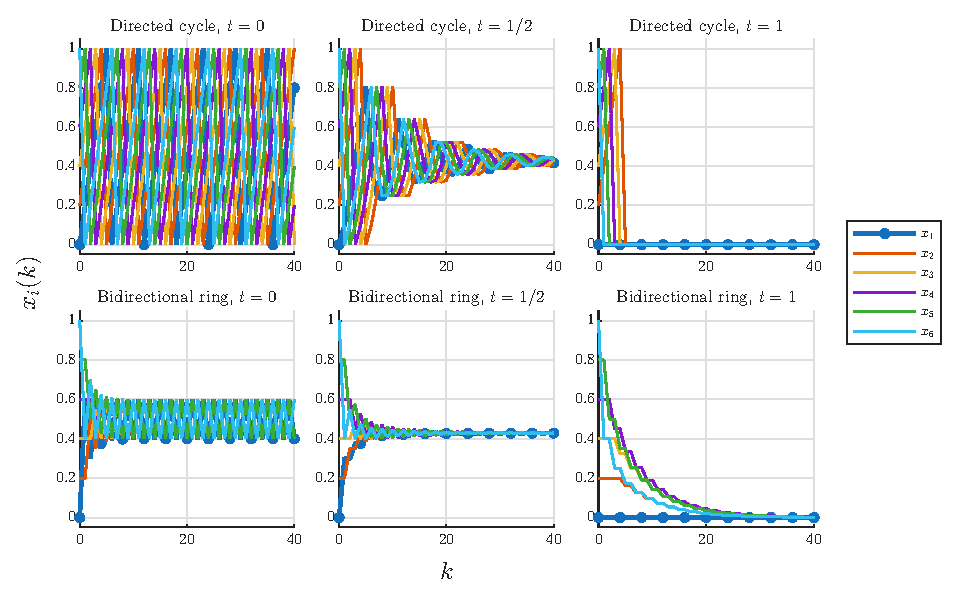
\includegraphics[width=0.94\textwidth]{figures/fdg_convergence.eps}
  \caption{Opinions $x_i(k)$ in the two networks of Figure~\ref{fig:networks}
  (top: directed cycle; bottom: bidirectional ring) for three values of the
  self-weight $t$ of agent~$1$ (columns), with
  $x(0) = (0,\, 0.2,\, 0.4,\, 0.6,\, 0.8,\, 1)^\top$. Agent~$1$ is marked with
  dots.}
  \label{fig:fdg-conv}
\end{figure}

In social terms, a group in which nobody gives weight to its own opinion can keep
passing opinions around forever; a single agent that gives some weight to its current
opinion, without being stubborn, is enough for the whole group to agree, and if that
agent becomes stubborn the agreement is on its own opinion. The network decides only
how this happens: by copying along a chain, or by averaging with the neighbours.
% REVISED (2026-10-28, review): shortened, same content. Was:
% In social terms, a group in which nobody gives weight to its own opinion can keep
% passing opinions around forever. It is enough that a single agent gives some weight to
% its current opinion, without being stubborn, for the whole group to reach an
% agreement. If that agent becomes stubborn, the agreement is reached on its own
% opinion. The structure of the network decides only how this happens: by copying along
% a chain in the directed cycle, by averaging with the neighbours in the bidirectional
% ring.

\subsubsection{Self-weights, stubbornness and social power}
\label{subsubsec:fdg-stub-power}

For $t > 0$ both networks reach a consensus (Section~\ref{subsubsec:fdg-stub-conv}),
so the social power $w$ of Section~\ref{subsubsec:consensus} is well defined, and
Theorem~\ref{thm:consensus} describes how it depends on $t$.
\begin{itemize}
  \item $0 < t < 1$: the digraph is strongly connected, so every agent is globally
        reachable and, by point~(i) of Theorem~\ref{thm:consensus}, every agent has a
        positive social power. Agent~$1$ gives weight to its own opinion, but it does
        not take all the influence: the initial opinion of every agent enters the
        consensus value.
  \item $t = 1$: agent~$1$ is stubborn and is the only globally reachable node, so
        $w = e_1$: the stubborn agent takes all the social power, and the initial
        opinions of the other agents have no effect on the final opinion of the group.
\end{itemize}

Between these two extremes, $w$ is the left eigenvector of $A(t)$ associated with the
eigenvalue $1$, normalized to sum $1$ (condition~(A2) of Theorem~\ref{thm:consensus});
Figure~\ref{fig:fdg-power} reports it for $t \in (0,1]$. Numerically, the social power
of agent~$1$ grows with $t$ towards $1$, while the other agents share the rest equally
($w_1 \approx 0.286$ and $w_i \approx 0.143$ for $i \neq 1$ when $t = 1/2$), with the
same values on the two networks. The bottom panel shows where the group converges, the
consensus value $w^\top x(0)$ (point~(ii) of Theorem~\ref{thm:consensus}): it moves
from the average $0.5$ of the initial opinions, for small $t$, to $x_1(0) = 0$ for
$t = 1$, and it is $\approx 0.429$ for $t = 1/2$, the value reached in
Figure~\ref{fig:fdg-conv}; also this curve is the same on the two networks. In other
words, on these two networks the self-weight of agent~$1$ changes how the opinions
converge, which depends on the network, but not where they converge.
% REVISED (2026-10-28, review): two paragraphs merged and shortened, same content. Was:
% Between these two extremes, the social power can be computed as the left eigenvector
% of $A(t)$ associated with the eigenvalue $1$, normalized so that its entries sum to $1$
% (condition~(A2) of Theorem~\ref{thm:consensus}). Figure~\ref{fig:fdg-power} reports
% the result for $t \in (0,1]$. Numerically, the social power of agent~$1$ grows with $t$
% towards $1$, while the other agents share the remaining social power equally; for
% $t = 1/2$, agent~$1$ has social power $\approx 0.286$ and every other agent
% $\approx 0.143$. Moreover, the computation gives the same values on the two networks.
% In other words, on these two networks the self-weight of agent~$1$ changes how the
% opinions converge, which depends on the network (Figure~\ref{fig:fdg-conv}), but not
% where they converge.
%
% The bottom panel of Figure~\ref{fig:fdg-power} shows where the group converges: by
% point~(ii) of Theorem~\ref{thm:consensus}, the consensus value is $w^\top x(0)$, here
% computed for $x(0) = (0,\, 0.2,\, 0.4,\, 0.6,\, 0.8,\, 1)^\top$, the initial condition of
% Figure~\ref{fig:fdg-conv}. For small $t$ all the agents have almost the same social
% power and the consensus value is close to the average of the initial opinions, $0.5$;
% as $t$ grows, the social power of agent~$1$ grows and the consensus value moves
% towards its initial opinion, $x_1(0) = 0$, which is reached for $t = 1$. For $t = 1/2$
% the consensus value is $\approx 0.429$, the value reached by the trajectories of
% Figure~\ref{fig:fdg-conv}. Also this curve is the same on the two networks.

\begin{figure}[H]
  \centering
  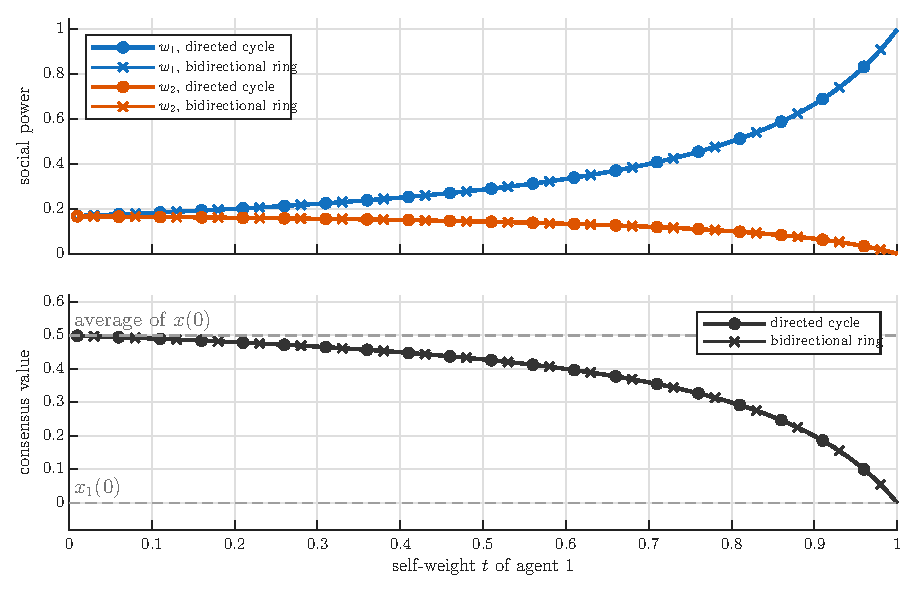
\includegraphics[width=0.94\textwidth]{figures/fdg_social_power.eps}
  \caption{Top: social power of agent~$1$ ($w_1$) and of agent~$2$ ($w_2$) as a
  function of the self-weight $t \in (0,1]$ of agent~$1$. Bottom: consensus value
  $w^\top x(0)$ for $x(0) = (0,\, 0.2,\, 0.4,\, 0.6,\, 0.8,\, 1)^\top$; the dashed
  lines mark the average of $x(0)$ and $x_1(0)$. Both panels are computed numerically
  in the directed cycle (dots) and in the bidirectional ring (crosses); the two networks
  give the same values.}
  \label{fig:fdg-power}
\end{figure}

\begin{remark}[More than one stubborn agent]
\label{rem:many-stubborn}
If two or more agents are stubborn, each of them is a sink of $C(G)$ made of a single,
aperiodic node. If every other agent is influenced, directly or through
intermediaries, by at least one stubborn agent, these are the only sinks, and by
Theorem~\ref{thm:disagreement} the group converges, but to a disagreement: every stubborn agent keeps its own initial opinion, and every other
agent converges to a convex combination of the opinions of the stubborn agents it is
influenced by (see also~\cite{proskurnikov2017tutorial}). Since there is no single
consensus value, the social power is no longer defined. This situation, in which
several agents are anchored to different fixed opinions, is the starting point of the
Friedkin--Johnsen model of Section~\ref{sec:fj}.
\end{remark}


% \input{fdg/...}

\section{FJ}
\label{sec:fj}

\subsection{Introduction to the FJ model}
\label{subsec:fj-intro}

\subsubsection{The FJ model}
\label{subsubsec:fj-model}

In the FDG model every agent keeps averaging the opinions it listens to, and a
persistent disagreement can only come from the structure of the network, i.e.\ from
several closed groups (Theorem~\ref{thm:disagreement}). The Friedkin--Johnsen (FJ)
model adds a second ingredient: each agent can also be tied to a fixed opinion of its own,
called its \emph{prejudice}. Following~\cite{proskurnikov2017tutorial}, the model reads
\begin{equation}\label{eq:fj}
  x(k+1) = \Lambda W x(k) + (I - \Lambda)\, u ,
\end{equation}
where
\begin{itemize}
  \item $W \in \mathbb{R}^{n \times n}$ is a row-stochastic matrix, the \emph{matrix of
        social influences}, i.e.\ the weighted adjacency matrix of the influence
        digraph $G$ (Definition~\ref{def:adjacency}), which plays the role of $A$ in
        the FDG model;
% REVISED (2026-10-28, review): the edge convention is already stated in Section 1.1. Was:
%   \item $W \in \mathbb{R}^{n \times n}$ is a row-stochastic matrix, the \emph{matrix of
%         social influences}, i.e.\ the weighted adjacency matrix of the influence
%         digraph $G$ (Definition~\ref{def:adjacency}); with the convention of
%         Section~\ref{subsec:prelim},
%         $w_{ij} > 0$ means that agent $i$ is influenced by agent $j$, so $W$ plays the
%         role that $A$ plays in the FDG model;
  \item $\Lambda = \operatorname{diag}(\lambda_1, \dots, \lambda_n)$, with
        $\lambda_i \in [0,1]$ the \emph{susceptibility} of agent $i$ to social
        influence;
  \item $u \in \mathbb{R}^n$ is a constant vector collecting the agents'
        \emph{prejudices}.
\end{itemize}
Componentwise,
\begin{equation}\label{eq:fj-i}
  x_i(k+1) = \lambda_i \sum_{j=1}^{n} w_{ij}\, x_j(k) + (1 - \lambda_i)\, u_i .
\end{equation}
At every step agent $i$ averages the opinions it listens to, exactly as in the FDG
model, and mixes this average with its prejudice: the weight $\lambda_i$ goes to the
others and the complement $1 - \lambda_i$ goes to $u_i$. The two quantities play
different roles: the prejudice $u_i$ is an opinion and says \emph{where} the agent is
anchored, while $1 - \lambda_i$ is a weight and says \emph{how strongly}. The model with
$u = x(0)$ appears in~\cite{bullo2024lns}, where $\lambda_i$ is called the openness
level of agent $i$ and $1 - \lambda_i$ its attachment to its initial opinion, which
plays the role of the prejudice.
% REVISED (2026-10-28, review): CORRECTION: the model of the book (Exercise E5.24) has u = x(0), it is not the same model with an independent u. Was:
% The same
% model appears in~\cite{bullo2024lns}, where $\lambda_i$ is called the openness level of
% agent $i$ and $1 - \lambda_i$ its attachment to the prejudice.

The special cases of~\eqref{eq:fj} are the following~\cite{proskurnikov2017tutorial}.
\begin{itemize}
  \item If $\lambda_i = 1$, agent $i$ follows the FDG rule. If $\Lambda = I$, the FJ
        model reduces to the FDG model with $A = W$; for this reason we assume
        $\Lambda \neq I$ from now on.
  \item If $\lambda_i < 1$, agent $i$ is called \emph{prejudiced}: it is anchored to its
        prejudice $u_i$.
  \item If $\lambda_i = 0$, then $x_i(k) = u_i$ for all $k \geq 1$: the agent ignores
        the others and jumps to its prejudice after one step. Its opinion never changes,
        i.e.\ the agent is stubborn in the sense of Definition~\ref{def:stubborn}, only
        if in addition $u_i = x_i(0)$. A stubborn agent of the FJ model is therefore an
        agent with $\lambda_i = 0$ and $u_i = x_i(0)$.
\end{itemize}

In social terms, the self-weight of the FDG model and the prejudice of the FJ model are
two different forms of resistance to influence. A self-weight ties an agent to its
\emph{current} opinion, which still moves towards the others
(Section~\ref{subsubsec:fdg-stub-model}); a prejudice ties it to a \emph{fixed}
opinion, which never moves.

In the original formulation of Friedkin and Johnsen the prejudices coincide with the
initial opinions, $u = x(0)$, and the susceptibilities are coupled to the self-weights
through $1 - \lambda_i = w_{ii}$~\cite{proskurnikov2017tutorial,bullo2024lns}. As
in~\cite{proskurnikov2017tutorial}, we do not impose these conditions: $u$ and $x(0)$
are independent, and so are $\Lambda$ and $W$. The choice $u = x(0)$ will be needed in
Section~\ref{subsubsec:fj-centrality} to define the influence centrality.

\subsubsection{Convergence and stability}
\label{subsubsec:fj-conv}
% RESTRUCTURED (2026-10-23): this subsubsection was called "Convergence: all agents
% P-dependent" and started from Corollary 22 of the tutorial. It now follows the order
% of the tutorial: definitions, P-dependent agents and decomposition, Theorem 21 (where
% V is defined), Corollary 22 (all agents P-dependent), Corollary 23, and only at the
% end our observations (error dynamics). The former subsubsection "The general case:
% P-independent agents" (label subsubsec:fj-general) is merged here.
% REVISED (2026-10-24): Definition P-dependent, Theorem 21, Corollaries 22 and 23 are
% now stated exactly as in the tutorial (only the notation is adapted); x(inf) = Vu is
% now outside Corollary 22, in eq. fj-V-all.
% REVISED (2026-10-23, after the general brainstorming): the observations are no longer
% in a separate block at the end; the intuition for Corollary 22 follows it directly,
% and Corollary 23 closes the subsubsection, as in the tutorial. The duplicated formula
% of V (former eq. fj-V-all before the corollary) is now only in the corollary. The
% version before this revision is saved in fj/fj_intro_OLD_2026-10-23.tex.

The FJ model~\eqref{eq:fj} is a linear system with the constant input $u$. Following
\cite{proskurnikov2017tutorial}, we say that it \emph{converges} if the limit
$x(\infty) = \lim_{k \to +\infty} x(k)$ exists for every initial condition $x(0)$, and
that it is \emph{asymptotically stable} if $\Lambda W$ is convergent, i.e.\
$\rho(\Lambda W) < 1$ (Definition~\ref{def:semiconv} and
Theorem~\ref{thm:spectral-radius}). Regular matrices are recalled in Definition~\ref{def:regular}.
% REVISED (2026-10-24): the prose definition of "regular" ("Following the same reference,
% a matrix A is called regular if ...") is replaced by Definition def:regular in the
% Preliminaries (Definition 15 of the tutorial).

Both properties are characterized by distinguishing the agents that are reached by the
prejudices from those that are not.

\begin{definition}[P-dependent agents~\cite{proskurnikov2017tutorial}]
\label{def:p-dependent}
Agent $i$ is \emph{P-dependent} if it is prejudiced or influenced by some prejudiced
agent $j$, that is, a walk from $i$ to $j$ in the graph $G$ exists. Otherwise, the
agent is \emph{P-independent}.
\end{definition}

The walk goes from the agent to the prejudiced agent because of our convention on the
edges; in~\cite{proskurnikov2017tutorial}, where the edges are drawn in the opposite
direction, the same walk goes from the prejudiced agent to the agent. In social terms,
an agent is P-dependent if at least one prejudice reaches it.

A P-independent agent $i$ is not prejudiced, so $\lambda_i = 1$, and it is not
influenced by any P-dependent agent: if $w_{ij} > 0$ with $j$ P-dependent, there would
be a walk from $i$ to a prejudiced agent through $j$, and $i$ would be P-dependent.
Since $\Lambda \neq I$, there is at least one prejudiced agent, hence at least one
P-dependent agent. Renumbering the agents so that agents $1, \dots, r$, with
$r \geq 1$, are P-dependent and agents $r+1, \dots, n$ are P-independent, and
splitting $x = [x^1; x^2]$, $u = [u^1; u^2]$, $W$ and $\Lambda$ accordingly, we
have $W^{21} = 0$ and $\Lambda^{22} = I$, and the model~\eqref{eq:fj} decomposes
as~\cite{proskurnikov2017tutorial}
\begin{align}
  x^1(k+1) &= \Lambda^{11}\bigl[W^{11} x^1(k) + W^{12} x^2(k)\bigr]
              + (I - \Lambda^{11})\, u^1, \label{eq:fj-dep}\\
  x^2(k+1) &= W^{22} x^2(k), \label{eq:fj-indep}
\end{align}
where $W^{22}$ is row-stochastic, since $W$ is row-stochastic and $W^{21} = 0$. The
P-independent agents therefore follow an FDG
model among themselves, with $A = W^{22}$, and no prejudice reaches them; the
P-dependent agents receive the opinions of the P-independent ones as an additional
input.

\begin{theorem}[\cite{proskurnikov2017tutorial}]
\label{thm:fj-general}
Let the community have $r \geq 1$ P-dependent agents and $n - r \geq 0$
P-independent ones. Then, the subsystem~\eqref{eq:fj-dep} is asymptotically stable,
i.e.\ $\Lambda^{11} W^{11}$ is Schur stable $\rho(\Lambda^{11} W^{11}) < 1$. The
model~\eqref{eq:fj} is convergent if and only if $r = n$ or~\eqref{eq:fj-indep} is
convergent, i.e.\ $W^{22}$ is regular. In this case
\begin{equation}\label{eq:fj-V}
  x^1(\infty) = V \begin{bmatrix} u^1 \\ x^2(\infty) \end{bmatrix}, \qquad
  V \triangleq (I_r - \Lambda^{11} W^{11})^{-1}
      \begin{bmatrix} I_r - \Lambda^{11} & \Lambda^{11} W^{12} \end{bmatrix}.
\end{equation}
The matrix $V$ is stochastic, i.e.\ the final opinion of any agent is a convex
combination of the prejudices and final opinions of P-independent agents.
\end{theorem}

In~\cite{proskurnikov2017tutorial}, \emph{stochastic} stands for row-stochastic in the
sense of Definition~\ref{def:row-stochastic}.

Theorem~\ref{thm:fj-general} can be read according to the number $r$ of P-dependent
agents.
\begin{itemize}
  \item $r = 0$. This case is not covered by Theorem~\ref{thm:fj-general}: no agent is
        prejudiced, i.e.\ $\Lambda = I$, and the FJ model~\eqref{eq:fj} reduces to the
        FDG model with $A = W$ (Section~\ref{subsec:fdg-intro}). This is why we assume
        $\Lambda \neq I$, which guarantees $r \geq 1$.
  \item $0 < r < n$. P-dependent and P-independent agents coexist. The P-independent
        agents follow~\eqref{eq:fj-indep}, which is an FDG model with the
        row-stochastic matrix $W^{22}$, so the outcomes of Table~\ref{tab:rosetta}
        apply to them. Denoting by $C^{22}$ the condensation digraph of the subgraph of
        P-independent agents, whose adjacency matrix is $W^{22}$, they reach
        \begin{itemize}
          \item a consensus, if $C^{22}$ has a unique sink, which is aperiodic
                (cases~(i) and~(iii));
          \item a disagreement, if $C^{22}$ has several sinks, all aperiodic
                (case~(iv));
          \item no convergence, if at least one sink of $C^{22}$ is periodic
                (cases~(ii) and~(v)).
        \end{itemize}
        In the first two cases $W^{22}$ is regular, the model~\eqref{eq:fj} converges
        and the final opinions of the P-dependent agents are given
        by~\eqref{eq:fj-V}; in the third case the model~\eqref{eq:fj} does not
        converge.
  \item $r = n$. There are no P-independent agents, the subsystem~\eqref{eq:fj-dep} is
        the whole model and the model~\eqref{eq:fj} always converges. This case is the
        subject of Corollary~\ref{cor:fj-stable} below.
\end{itemize}
In social terms, the P-dependent agents settle on a compromise between the prejudices
and the opinions of the P-independent agents they listen to whenever these opinions
settle; whether the whole group settles is decided only by the P-independent agents.
% REVISED (2026-10-24): reading of Theorem 21 organized by the number r of P-dependent
% agents (r = 0: FDG, excluded; 0 < r < n: outcomes of Table 1 for the P-independent
% agents; r = n: Corollary 22). The symbol C^{22} is ours.


\begin{corollary}[\cite{proskurnikov2017tutorial}]
\label{cor:fj-stable}
The Friedkin--Johnsen model~\eqref{eq:fj} is asymptotically stable if and only if all
agents are P-dependent. Then, $V = (I - \Lambda W)^{-1}(I - \Lambda)$. This holds, in
particular, if $\Lambda < I_n$ or $\Lambda \neq I_n$ and $G$ is strongly connected
($W$ is irreducible).
\end{corollary}

With $r = n$,~\eqref{eq:fj-V} gives, for every $x(0)$,
\begin{equation}\label{eq:fj-V-all}
  x(\infty) = V u ,
\end{equation}
with $V$ as in Corollary~\ref{cor:fj-stable}.

The condition of Corollary~\ref{cor:fj-stable} can also be read on the matrix
$\Lambda W$ with the tools of the course. The matrix $\Lambda W$ is no longer
row-stochastic: since $W$ is row-stochastic, the $i$-th row of $\Lambda W$ sums to
$\lambda_i$. Rows of agents that are not prejudiced sum to $1$, rows of prejudiced
agents sum to less than $1$, and since $\Lambda \neq I$ at least one such row exists.
Hence $\Lambda W$ is row-substochastic (Definition~\ref{def:row-substochastic}) and
Lemma~\ref{lem:substochastic} applies.
% MOVED (2026-10-23): Definition "Row-substochastic matrix" and Lemma "Convergent
% row-substochastic matrices" were here; they are now in the Preliminaries
% (Section 1.1.2), with the definition of weighted out-degree.

For the matrix $\Lambda W$, the weighted out-degree of agent $i$ is $\lambda_i$: the nodes with
out-degree $1$ are the agents that are not prejudiced, and the nodes with out-degree
less than $1$ are the prejudiced agents. The condition of
Lemma~\ref{lem:substochastic} therefore reads: every agent that is not prejudiced is
influenced, directly or through intermediaries, by a prejudiced agent, i.e.\ all the
agents are P-dependent. This is exactly the condition of
Corollary~\ref{cor:fj-stable}. Indeed,~\cite{proskurnikov2017tutorial} remarks that
Corollary~\ref{cor:fj-stable} can be turned into a criterion of Schur stability for
substochastic matrices, and~\cite{bullo2024lns} proves the same condition for the FJ
model through this lemma.

Two observations of ours give an intuition for Corollary~\ref{cor:fj-stable}. First,
letting $k \to +\infty$ in~\eqref{eq:fj} shows that the limit $x(\infty) = Vu$ is an
equilibrium, $x(\infty) = \Lambda W x(\infty) + (I - \Lambda)u$. Letting
$e(k) = x(k) - x(\infty)$ and subtracting this equation from~\eqref{eq:fj} gives
\begin{equation}\label{eq:fj-error}
  e(k+1) = \Lambda W\, e(k),
\end{equation}
an autonomous linear system in which the prejudice $u$ does not appear: $\Lambda W$
decides whether the opinions converge, $u$ decides where.

Second, the linear system~\eqref{eq:fj-error} shows the role of the P-dependent
agents. At each step, agent $i$ keeps a fraction $\lambda_i$ of the weighted average
of the deviations of the agents it listens to. An agent that is not prejudiced
($\lambda_i = 1$) only averages the deviations, while a prejudiced agent loses a
fraction $1-\lambda_i$ of them (in~\eqref{eq:fj}, this fraction is replaced by the
agent's fixed prejudice). The deviations therefore leave the group only through the
prejudiced agents, and they vanish only if every agent is influenced, directly or
through intermediaries, by one of them, i.e.\ all agents are P-dependent. A group of
agents that is not influenced, even indirectly, by any prejudiced agent loses no
deviation and behaves as an FDG model, as in~\eqref{eq:fj-indep}.

In social terms, the group converges, for every initial opinion, as soon as every agent
that is not anchored to a prejudice listens, directly or through intermediaries, to
someone who is. On a strongly connected network, such as the two networks of
Figure~\ref{fig:networks}, a single prejudiced agent is enough. Note that this does not
require aperiodicity, unlike the FDG model of Section~\ref{subsec:fdg-stub}.

If some agents are P-independent, the model is not asymptotically stable, but it may
still converge. Theorem~\ref{thm:fj-general} gives the condition in terms
of $W^{22}$; in terms of the whole matrix $\Lambda W$ it reads as follows.

\begin{corollary}[\cite{proskurnikov2017tutorial}]
\label{cor:fj-regular}
The model~\eqref{eq:fj} converges if and only if $\Lambda W$ is regular, i.e.\ the
limit $\lim_{k \to \infty} (\Lambda W)^k$ exists.
\end{corollary}

As remarked in~\cite{proskurnikov2017tutorial}, this property is not trivial: a system
$x(k+1) = A x(k) + B u$ with a regular matrix $A$ may not converge, and may even have
unbounded solutions, as for $A = B = I$.

\subsubsection{How the opinions converge: the matrix \texorpdfstring{$V$}{V} and the augmented graph}
\label{subsubsec:fj-final}
% RENAMED (2026-10-24): was "Final opinions: consensus or disagreement" -- the tutorial
% does not use consensus/disagreement for the FJ model (Section 6); consensus
% (Definition 14 of the tutorial) is a property of the FDG model.
% RENAMED (2026-10-23): was "The equilibrium and the augmented graph"
% (label subsubsec:fj-equilibrium).

When all agents are P-dependent, the final opinions are given
by~\eqref{eq:fj-V-all}, and the convex combination of Theorem~\ref{thm:fj-general}
involves only the prejudices:
\[
  x_i(\infty) = \sum_{j=1}^{n} v_{ij}\, u_j .
\]
Three facts follow.
\begin{itemize}
  \item The initial opinions are forgotten: $x(0)$ does not appear in $x(\infty)$.
  \item Only the prejudices of prejudiced agents count: if $\lambda_j = 1$, the $j$-th
        column of $I - \Lambda$ is zero, hence so is the $j$-th column of $V$, and
        $u_j$ has no weight in any final opinion.
  \item Every final opinion lies between the smallest and the largest prejudice of the
        prejudiced agents.
\end{itemize}
The comparison with the FDG model is instructive. There, the consensus value
$w^\top x(0)$ is a weighted average of the initial opinions, with the same weights $w$
for every agent (Theorem~\ref{thm:consensus}); here, the final opinions are weighted
averages of the prejudices, and each agent has its own weights, given by its row of
$V$.

In the FDG model, consensus is a property of the model: the model reaches a consensus
if the final opinions coincide for any initial condition
$x(0)$~\cite{proskurnikov2017tutorial}. In the FJ model with all agents P-dependent,
the limit $x(\infty) = Vu$ does not depend on $x(0)$
(equation~\eqref{eq:fj-V-all}): whether the final opinions coincide is decided by the
prejudices $u$, which are an external input, through the matrix $V$, and no longer by
the initial opinions. In our
reading, this is why~\cite{proskurnikov2017tutorial} studies the FJ model in terms of convergence and
of the form of the limit, and not in terms of consensus.
% REVISED (2026-10-24): was "...decided by the prejudices u, which are an external
% input, and not by the network" -- false in general: with a single prejudiced agent
% V = 1 e_1^T (V row-stochastic, zero columns for lambda_j = 1) and the final opinions
% coincide for every u (Section 3.2.2), so the network matters too.

The notion of consensus of the FDG model applies again only to the P-independent agents
($0 < r < n$), which evolve as an FDG model with matrix $W^{22}$ and whose limit depends
on their initial opinions $x^2(0)$ (Section~\ref{subsubsec:fj-conv}). The P-dependent
agents converge to convex combinations of the prejudices and of the final opinions of
the P-independent agents (Theorem~\ref{thm:fj-general}), so they do not necessarily end
up at the consensus value of the P-independent agents, even when there is one.
% REVISED (2026-10-28, review): shortened: the three outcomes for the P-independent agents are already listed in Section 3.1.2. Was:
% The notion of consensus of the FDG model applies again only when some agents are
% P-independent ($0 < r < n$), and only to them. These agents are not prejudiced and are
% not influenced by any P-dependent agent, so they evolve as an FDG model with matrix
% $W^{22}$ (equation~\eqref{eq:fj-indep}), and their limit depends on their initial
% opinions $x^2(0)$. For them, the three outcomes of the FDG model are possible:
% consensus, disagreement or no convergence (Table~\ref{tab:rosetta}). The P-dependent
% agents, instead, converge to convex combinations of the prejudices and of the final
% opinions of the P-independent agents (Theorem~\ref{thm:fj-general}); hence, even if
% the P-independent agents reach a consensus among themselves, the P-dependent agents do
% not necessarily end up at the same value.

The limit~\eqref{eq:fj-V-all} has a direct interpretation in terms of the FDG model.
Following~\cite{proskurnikov2017tutorial}, the FJ model~\eqref{eq:fj} may be
considered as an augmented FDG model with $n$ virtual stubborn agents, anchored at the
prejudices: the virtual agent $i'$ associated with agent $i$ keeps the opinion
$x_{i'}(k) = u_i$ for all $k$. Explicitly (this rewriting is ours), stacking the
opinions $x$ of the real agents and $x'$ of the virtual agents,
\begin{equation}\label{eq:fj-augmented}
  \begin{bmatrix} x(k+1) \\ x'(k+1) \end{bmatrix}
  = \begin{bmatrix} \Lambda W & I - \Lambda \\ 0 & I \end{bmatrix}
    \begin{bmatrix} x(k) \\ x'(k) \end{bmatrix},
  \qquad x'(0) = u .
\end{equation}
Row $i$ of the matrix in~\eqref{eq:fj-augmented} sums to $\lambda_i + (1-\lambda_i) = 1$,
and row $i'$ sums to $1$; hence the matrix is row-stochastic
and~\eqref{eq:fj-augmented} is an FDG model on $2n$ agents. In its digraph, which we
call the \emph{augmented graph}:
\begin{itemize}
  \item a real agent $i$ is influenced by a real agent $j$ with weight
        $\lambda_i w_{ij}$;
  \item a real agent $i$ is influenced by its virtual agent $i'$ with weight
        $1 - \lambda_i$, so this edge exists only if agent $i$ is prejudiced;
  \item a virtual agent $i'$ is influenced only by itself, with weight $1$, so its
        opinion never changes: it is stubborn (Definition~\ref{def:stubborn}).
\end{itemize}
Figure~\ref{fig:augmented} shows the FJ model on the directed cycle of
Figure~\ref{fig:networks}(a) when agent~$1$ is the only prejudiced agent, and the
corresponding augmented graph. In panel~(a) the prejudice is drawn as an input
entering agent~$1$, since it is not an agent of the network but an external piece of
information; in panel~(b) it becomes the virtual agent $1'$, and the edge follows our
convention: it goes from $1$ to $1'$, because agent~$1$ listens to $1'$. In social
terms, a prejudice behaves as an additional agent that never changes its opinion: a
prejudiced agent keeps listening to the others, and also listens to this stubborn
agent placed beside it.

\begin{figure}[H]
  \centering
  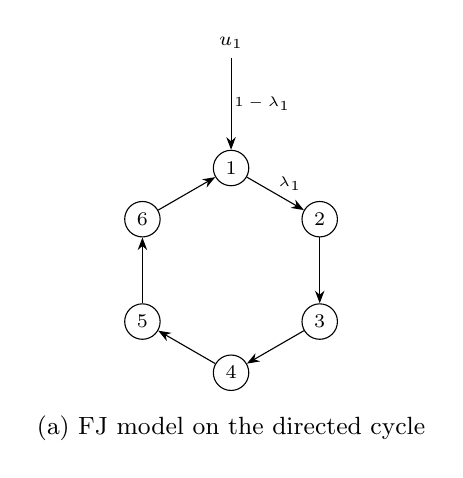
\begin{tikzpicture}[baseline=(c.base)]
    \foreach \i in {1,...,6} {
      \node[agent] (p\i) at ({90-60*(\i-1)}:1.3) {\i};
    }
    \node (c) at (0,0) {};
    \foreach \i/\j in {2/3,3/4,4/5,5/6,6/1} {
      \draw[edge] (p\i) -- (p\j);
    }
    \draw[edge] (p1) -- node[weight, above right] {$\lambda_1$} (p2);
    \draw[edge] (0,2.7) node[above, font=\scriptsize] {$u_1$}
      -- node[weight, right] {$1-\lambda_1$} (p1);
    \node at (0,-2.0) {\small (a) FJ model on the directed cycle};
  \end{tikzpicture}
  \hspace{1.5cm}
  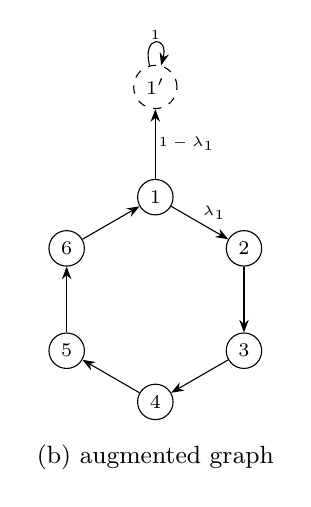
\begin{tikzpicture}[baseline=(c.base)]
    \foreach \i in {1,...,6} {
      \node[agent] (a\i) at ({90-60*(\i-1)}:1.3) {\i};
    }
    \node (c) at (0,0) {};
    \foreach \i/\j in {2/3,3/4,4/5,5/6,6/1} {
      \draw[edge] (a\i) -- (a\j);
    }
    \draw[edge] (a1) -- node[weight, above right] {$\lambda_1$} (a2);
    \node[agent, dashed, minimum size=5.5mm] (v1) at (0,2.7) {$1'$};
    \draw[edge] (a1) -- node[weight, right] {$1-\lambda_1$} (v1);
    \draw[selfloop] (v1) to node[weight, above] {$1$} (v1);
    \node at (0,-2.0) {\small (b) augmented graph};
  \end{tikzpicture}
  \caption{The FJ model on the directed cycle of Figure~\ref{fig:networks}(a) when
  agent~$1$ is the only prejudiced agent ($\lambda_1 < 1$, $\lambda_i = 1$ for
  $i \neq 1$), and its augmented graph. Unlabelled edges have weight $1$. (a)~The
  prejudice $u_1$ enters agent~$1$ as an external input, with weight $1-\lambda_1$;
  this arrow is not an edge of $G$. (b)~The input becomes the virtual agent $1'$
  (dashed), which is stubborn and keeps the opinion $u_1$. The virtual agents
  $2', \dots, 6'$ are stubborn agents that nobody listens to, and are not drawn.}
  \label{fig:augmented}
\end{figure}
% REVISED (2026-10-24): Figure fig:augmented now has two panels, (a) the FJ model with
% the prejudice as an input arrow entering agent 1 and (b) the augmented graph
% (option (a) chosen by the user; the change of direction is explained in the text).

The augmented graph also shows, from the side of the FDG model, why consensus is not
the right notion for the FJ model. This observation is ours. The augmented
model~\eqref{eq:fj-augmented} is an FDG model, so the classification of
Table~\ref{tab:rosetta} applies to it. Each virtual agent is influenced only by
itself, so it is a sink of the condensation digraph of the augmented graph, and it is
aperiodic because of its self-loop. Hence the augmented graph has at least $n$ sinks
and it is not strongly connected; for $n \geq 2$, the consensus cases~(i) and~(iii) of
Table~\ref{tab:rosetta} never occur, and neither does case~(ii). Only two outcomes
remain.
\begin{itemize}
  \item \emph{Disagreement} (case~(iv)), when all the sinks are aperiodic. If all
        agents are P-dependent, the only sinks are the $n$ virtual agents, since every
        real agent is influenced, directly or through intermediaries, by some
        prejudiced agent $j$, and hence by $j'$. This is the situation of
        Remark~\ref{rem:many-stubborn}: by Theorem~\ref{thm:disagreement}, every real
        agent converges to a convex combination of the opinions of the stubborn
        virtual agents, i.e.\ of the prejudices, which is
        exactly~\eqref{eq:fj-V-all}. If some agents are P-independent, the sinks of
        $C^{22}$ are further sinks of the augmented graph, and all of them are
        aperiodic if and only if $W^{22}$ is regular.
  \item \emph{No convergence} (case~(v)), when at least one sink of $C^{22}$ is
        periodic, i.e.\ when $W^{22}$ is not regular.
\end{itemize}
These two outcomes are exactly the two alternatives of
Theorem~\ref{thm:fj-general}. The disagreement of case~(iv) concerns all the $2n$ agents
of the augmented model, whose virtual agents keep their different values $u_i$ forever
($x'(0) = u$ is part of the initial condition); it does not imply that the final
opinions of the real agents differ, which, as discussed above, depends on $V$ and $u$.
% REVISED (2026-10-28, review): shortened, same content. Was:
% These two outcomes are exactly the two alternatives of
% Theorem~\ref{thm:fj-general}. Note that the disagreement of case~(iv) concerns all the
% $2n$ agents of the augmented model: the virtual agents keep their different values
% $u_i$ forever, because in the augmented model the prejudices are part of the initial
% condition, $x'(0) = u$. It does not imply that the final opinions of the real agents
% differ, which, as discussed above, depends on $V$ and $u$.
% REVISED (2026-10-24): was "depends on u" (see the REVISED note above).
% NOTE (2026-10-24): footnote 21 of the tutorial (stubbornness as part of the state in
% the FDG model vs external input in the FJ model) goes to Section 3.2.1.

% TODO (to study before writing): the augmented graph~\cite{proskurnikov2017tutorial}:
% each prejudice u_i as a virtual stubborn agent anchored at u_i; TikZ figure; link with
% Remark rem:many-stubborn (several stubborn agents -> disagreement in the FDG model).
% TODO (OURS, R6, may be discarded): augmented graph = case (iv) of the Rosetta stone.
% TODO (to study with the simulations): consensus or disagreement. Sources: Bullo E5.24(v)
% (V_1 = [1 0; 1 0]: one prejudiced agent -> consensus; V_2: disagreement "for generic
% initial opinions"), tutorial Example 3 (cleavage). Consequences of V row-stochastic +
% zero columns (ours): one prejudiced agent, or equal prejudices of all prejudiced
% agents -> consensus. No general rule in the sources. Contrast with the FDG model
% (disagreement only from >= 2 sinks).
% DONE (2026-10-24): the TODOs above are written in the text, with the augmented graph,
% Figure fig:augmented, the consensus discussion (tutorial Definition 14) and our
% reading via Table 1 (R6). Excluded on purpose: Bullo E5.24(v) and the rule "one
% prejudiced agent <-> consensus" (not in the tutorial).

\subsubsection{Influence centrality}
\label{subsubsec:fj-centrality}

% TODO (to study before writing): influence centrality~\cite{proskurnikov2017tutorial}:
% asymptotically stable model and u = x(0), c = n^{-1} V^T 1_n (mean weight of x_i(0) in
% the final opinions), c^T 1_n = 1; Lemma 24 (Lambda = alpha I, alpha -> 1: c_alpha ->
% French's social power); possibly Bullo E5.24(iv) (Lambda = lambda I: A and V have the
% same left dominant eigenvector).
% DONE (2026-10-24): written below from Section 6.2 of the tutorial. Excluded on purpose:
% PageRank (not about social networks) and the reading of c on the augmented graph.

In the FDG model the social power $w$ is defined only when the group reaches a
consensus (Section~\ref{subsubsec:consensus}), which is not the relevant notion for the
FJ model (Section~\ref{subsubsec:fj-final}). Nor does the augmented FDG
model~\eqref{eq:fj-augmented} help: its graph has at least $n$ sinks, so for $n \geq 2$
it never reaches a consensus and its social power is not defined (this remark is ours). A different measure is needed,
and~\cite{proskurnikov2017tutorial} discusses an extension of the social power to the FJ
model, introduced by Friedkin.
% REVISED (2026-10-28, review): shortened; the n sinks of the augmented graph are shown in Section 3.1.3. Was:
% In the FDG model, the social power $w$ measures the weight of each initial opinion in
% the consensus value, and it is defined only when the group reaches a consensus
% (Section~\ref{subsubsec:consensus}). In the FJ model consensus is not the relevant
% notion (Section~\ref{subsubsec:fj-final}), so the social power cannot be used as it
% is. Rewriting the FJ model as the augmented FDG model~\eqref{eq:fj-augmented} does not
% help: the augmented graph has at least $n$ sinks, so for $n \geq 2$ the augmented
% model never reaches a consensus and its social power is not defined (this remark is ours). A
% different measure is needed:~\cite{proskurnikov2017tutorial} discusses an extension of
% the social power to the FJ model, introduced by Friedkin.

\paragraph{Influence centrality.}
As in~\cite{proskurnikov2017tutorial}, we confine ourselves to the asymptotically
stable FJ model with $u = x(0)$, the traditional assumption of the Friedkin--Johnsen
theory (Section~\ref{subsubsec:fj-model}); then $x(\infty) = V x(0)$
by~\eqref{eq:fj-V-all}. The assumption $u = x(0)$ is what gives the initial
opinions a role: in general $x(\infty) = Vu$ does not depend on $x(0)$, so the initial
opinions would have no weight in the final opinions. The social power of agent $i$ is
generalized as the mean weight of its initial opinion in determining the group
members' final opinions~\cite{proskurnikov2017tutorial}. These mean weights are the
elements of the non-negative vector $c$ such that
\begin{equation}\label{eq:influence}
  c = n^{-1} V^\top \mathbf{1}_n, \qquad
  \bar x = \frac{1}{n} \sum_{i=1}^{n} x_i(\infty)
         = \frac{1}{n} \mathbf{1}_n^\top V x(0) = c^\top x(0),
\end{equation}
and $c_i$ is called the \emph{influence centrality} of agent
$i$~\cite{proskurnikov2017tutorial}. In terms of $V$, $c_i$ is the average of the
$i$-th column of $V$, whose entries are the weights of $x_i(0)$ in the final opinions
of the single agents. Since $V$ is stochastic, $c$ is non-negative and $c^\top \mathbf{1}_n = 1$, like $w$
(Theorem~\ref{thm:consensus}), so the two measures can be compared directly. Similar to
French's social power, the influence centrality is generated by an opinion formation
mechanism~\cite{proskurnikov2017tutorial}.
% REVISED (2026-10-28, review): "sums to 1" was said twice. Was:
% Since $V$ is stochastic, $c^\top \mathbf{1}_n = 1$, and, similar
% to French's social power, the influence centrality is generated by an opinion
% formation mechanism~\cite{proskurnikov2017tutorial}. Like $w$ (Theorem~\ref{thm:consensus}),
% the vector $c$ is non-negative and sums to $1$, so the two measures can be compared
% directly.

The relation with the social power is made precise in~\cite{proskurnikov2017tutorial}.
The convergence and the consensus of the FDG model are equivalent, respectively, to
the regularity and the full regularity of the stochastic matrix
$A$~\cite{proskurnikov2017tutorial} (Definition~\ref{def:regular}). For a fixed $W$,
let $\Lambda = \alpha I_n$ with $\alpha \in (0,1)$, i.e.\ the same susceptibility for
all agents, and consider the corresponding matrix $V_\alpha$ and vector $c_\alpha$.
For $\alpha = 0$, i.e.\ $\Lambda = 0$, every agent keeps its initial opinion, $V = I$
and $c_0 = n^{-1} \mathbf{1}_n$: the social power is uniformly distributed between all
agents~\cite{proskurnikov2017tutorial}.

\begin{lemma}[\cite{proskurnikov2017tutorial}]
\label{lem:centrality-limit}
Let $W$ be a fully regular matrix and $w$ stand for the vector of French's social
power, corresponding to the FDG model~\eqref{eq:fdg} with $A = W$. Then,
$w = \lim_{\alpha \to 1-0} c_\alpha$.
\end{lemma}

The limit cannot be replaced by $\alpha = 1$: for $\Lambda = I$ the FJ model is the
FDG model, which is not asymptotically stable, and $I - W$ is singular since
$1 \in \operatorname{spec}(W)$ (Theorem~\ref{thm:stoch-spectrum}), so $V$ is not
defined. In social terms, the influence centrality moves from the uniform
distribution, when every agent is anchored to its own initial opinion, to French's
social power, when the weight of the prejudices vanishes.

% REMOVED (2026-10-23): \subsubsection{The general case: P-independent agents}
% \label{subsubsec:fj-general} -- merged into Section 3.1.2 (Theorem 21 and
% Corollary 23 of the tutorial), to follow the order of the tutorial.



\subsection{Stubborness and social power in the FJ model}


% \input{fj/...}

\section{Conclusions}
\label{sec:conclusions}

% \input{conclusion/...}


\bibliographystyle{plain}
\bibliography{references}

\end{document}
